%\title{LaTeX Portrait Poster Template}
%%%%%%%%%%%%%%%%%%%%%%%%%%%%%%%%%%%%%%%%%
% a0poster Portrait Poster
% LaTeX Template
% Version 1.0 (22/06/13)
%
% The a0poster class was created by:
% Gerlinde Kettl and Matthias Weiser (tex@kettl.de)
% 
% Adapter by Jens Buysse for Hogeschool Gent
% This template has been downloaded from:
% http://www.LaTeXTemplates.com
%
% License:
% CC BY-NC-SA 3.0 (http://creativecommons.org/licenses/by-nc-sa/3.0/)
%
%%%%%%%%%%%%%%%%%%%%%%%%%%%%%%%%%%%%%%%%%

%----------------------------------------------------------------------------------------
%	PACKAGES AND OTHER DOCUMENT CONFIGURATIONS
%----------------------------------------------------------------------------------------

\documentclass[a0,portrait]{a0poster}

\usepackage{multicol} % This is so we can have multiple columns of text side-by-side
\columnsep=100pt % This is the amount of white space between the columns in the poster
\columnseprule=3pt % This is the thickness of the black line between the columns in the poster

\usepackage[svgnames]{xcolor} % Specify colors by their 'svgnames', for a full list of all colors available see here: http://www.latextemplates.com/svgnames-colors

\usepackage{times} % Use the times font
%\usepackage{palatino} % Uncomment to use the Palatino font

\usepackage{graphicx} % Required for including images
\graphicspath{{figures/}} % Location of the graphics files
\usepackage{booktabs} % Top and bottom rules for table
\usepackage[font=small,labelfont=bf]{caption} % Required for specifying captions to tables and figures
\usepackage{amsfonts, amsmath, amsthm, amssymb} % For math fonts, symbols and environments
\usepackage{wrapfig} % Allows wrapping text around tables and figures
\usepackage[export]{adjustbox}

\begin{document}

%----------------------------------------------------------------------------------------
%	POSTER HEADER 
%----------------------------------------------------------------------------------------

% The header is divided into two boxes:
% The first is 75% wide and houses the title, subtitle, names, university/organization and contact information
% The second is 25% wide and houses a logo for your university/organization or a photo of you
% The widths of these boxes can be easily edited to accommodate your content as you see fit

\begin{minipage}[t]{0.75\linewidth}
\VeryHuge \color{HoGentAccent1} \textbf{Ontwikkeling van de Proof of Concept voor een nieuw IT asset management programma voor AZ Glorieux gebouwd met Power Apps.} \color{Black}\\ % Title
%\Huge\textit{Ondertitel (eventueel)}\\[2.4cm] % Subtitle

\huge \textbf{Van den Hauwe Thomas, Vanneste Siemen, Vertonghen Benjamin}\\[0.5cm] % Author(s)
\huge Hogeschool Gent, Valentin Vaerwyckweg 1, 9000 Gent\\[0.4cm] % University/organization
\Large \texttt{thomas.vandenhauwe.v7877@hogent.be} \\
\end{minipage}
%
\begin{minipage}[t]{0.25\linewidth}

\includegraphics[width=13cm,right]{figures/HOGENT_Logo_Pos_rgb.png} 

\end{minipage}

\vspace{1cm} % A bit of extra whitespace between the header and poster content

%----------------------------------------------------------------------------------------

\begin{multicols}{2} % This is how many columns your poster will be broken into, a portrait poster is generally split into 2 columns

%----------------------------------------------------------------------------------------
%	ABSTRACT
%----------------------------------------------------------------------------------------

\color{HoGentAccent1} % Navy color for the abstract

\begin{abstract}
Het ziekenhuis AZ Glorieux zou graag PowerApps willen gebruiken om een oude business applicatie (LanReview, ITAM) te vervangen. Specifiek wordt bekeken hoe geschikt PowerApps is voor deze rol.\\
Dit onderzoek is relevant omdat het algemene zakelijke landschap gekenmerkt is door een ontoereikendheid aan de vraag om software en het is interessant om te zien of low-code zijn beloofde snellere softwareontwikkeling kan waarmaken. 

Eerst wordt de omgeving van AZ Glorieux verkend en wordt LanReview in detail besproken. Het begrip low-code wordt onderzocht, in het bijzonder wordt er een actueel beeld van geschetst. Het PowerApps platform wordt onder de loep genomen.

Er wordt een requirementsanalyse gemaakt. De low-code markt wordt onderzocht en met de requirements in het achterhoofd wordt er een low-code (voor powerusers) platform gekozen voor de primaire proof-of-concept en hierna een low-code (voor ontwikkelaars) platform voor de secundaire proof-of-concept. Dit zijn PowerApps en Outsystems geworden.

In de volgende delen worden de proof-of-concepts voor beiden uitgewerkt. Dit wordt gedaan door elke requirement te implementeren en te documenteren.

Tenslotte komt het besluit dat PowerApps niet de beste optie is voor deze case en wordt genuanceerd voor wat het wel en niet geschikt zou zijn. Dit wordt gedaan voor zowel PowerApps (no-code) als Outsystems (low-code).
\end{abstract}
%----------------------------------------------------------------------------------------
%	INTRODUCTION
%----------------------------------------------------------------------------------------

\color{HoGentAccent1} 
\section*{Introductie}
\color{black}
\color{black}
LanReview, een binnenshuis ontwikkeld assetmanagement programma dat onontbeerlijk is voor de IT Helpdesk van het ziekenhuis AZ Glorieux, is aan vernieuwing toe. De laatste ontwikkeling is van enige tijd geleden en het is niet logisch meer om dit terug op te nemen voornamelijk wegens de verouderde codebase (Visual BASIC 3.0). De vervangende applicatie moet bij voorkeur gemaakt worden met Microsoft Power Apps en ondersteunend ook Power Automate. De vraag wordt met andere woorden gesteld wat voor potentieel dit platform heeft en hoe het past in hun omgeving.\\
Dit is op zich niet speciaal. Bedrijven kampen al jaren met een niet in te vullen vraag naar software en dit zal in de toekomst alleen maar blijven toenemen. Low-code platformen (waaronder het Microsoft Power platform) stellen zichzelf als het beste gereedschap om dit probleem aan te pakken.\\
Dat is wat onderzocht zal worden. Specifiek wordt gekeken hoe gepast het PowerApps gereedschap is om het LanReview probleem op te lossen. Dit wordt gedaan aan de hand van een proof-of-concept.

%\begin{center}\vspace{1cm}
%    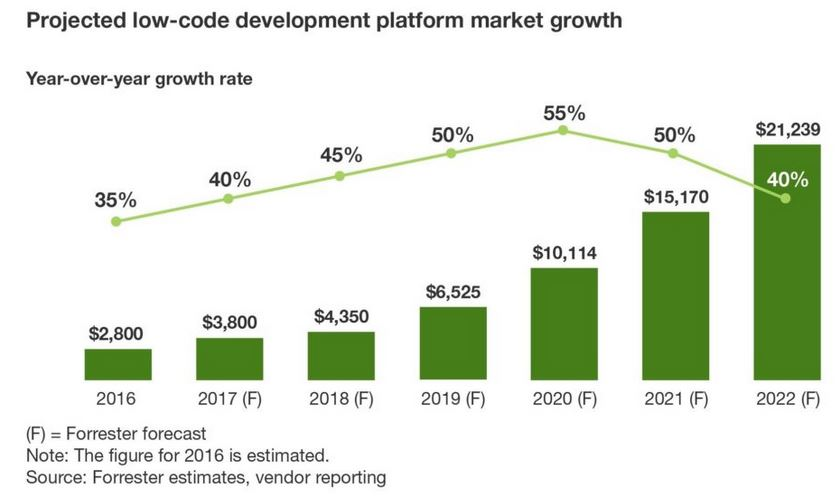
\includegraphics[width=0.7\linewidth]{forrester-markt-evolutie}
%    \captionof{figure}{\color{HoGentAccent5} Forrester voorspelde marktevolutie.}
%\end{center}\vspace{1cm}

%----------------------------------------------------------------------------------------
%	GEOLOGY
%----------------------------------------------------------------------------------------

\color{Black} % DarkSlateGray color for the rest of the content
\color{HoGentAccent1} 
\section*{Experimenten}
\color{black}
\begin{itemize}
    \item Requirementsanalyse:\\
    Het hoofddoel was om een eerste peiling te doen naar de geschiktheid van PowerApps en het ontdekken van het beste platform om de secundaire proof-of-concept mee te bouwen. Er wordt traditioneel te werk gegaan: prioriteiten stellen onder de requirements, longlist en shortlist.
    \item Proof-of-concept: Power Apps\\
    %Dit werd gedaan door de requirements uit te werken en hun voldoening te bekijken.
    De requirements worden uitgewerkt en gedocumenteerd. Er wordt noot genomen van de mate van voldoening.
    \item Proof-of-concept: Outsystems\\
    %Dezelfde werkwijze is gebruikt.
    De vorige werkwijze wordt ook hier op dezelfde manier toegepast.
\end{itemize}


\color{HoGentAccent1} 
\section*{Sectie met figuur}
\color{black}


\begin{center}\vspace{1cm}
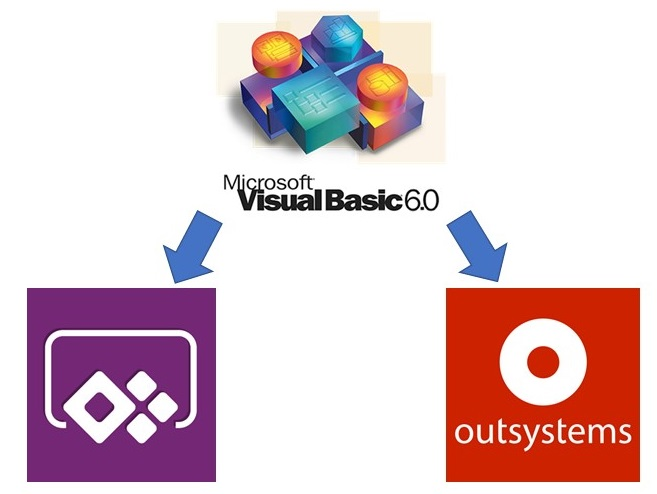
\includegraphics[width=0.7\linewidth]{plat-tri}
\captionof{figure}{\color{HoGentAccent5} Een overzicht van de gerbuikte platformen, PowerApps en Outsystems.}
\end{center}\vspace{1cm}

\begin{center}\vspace{1cm}
    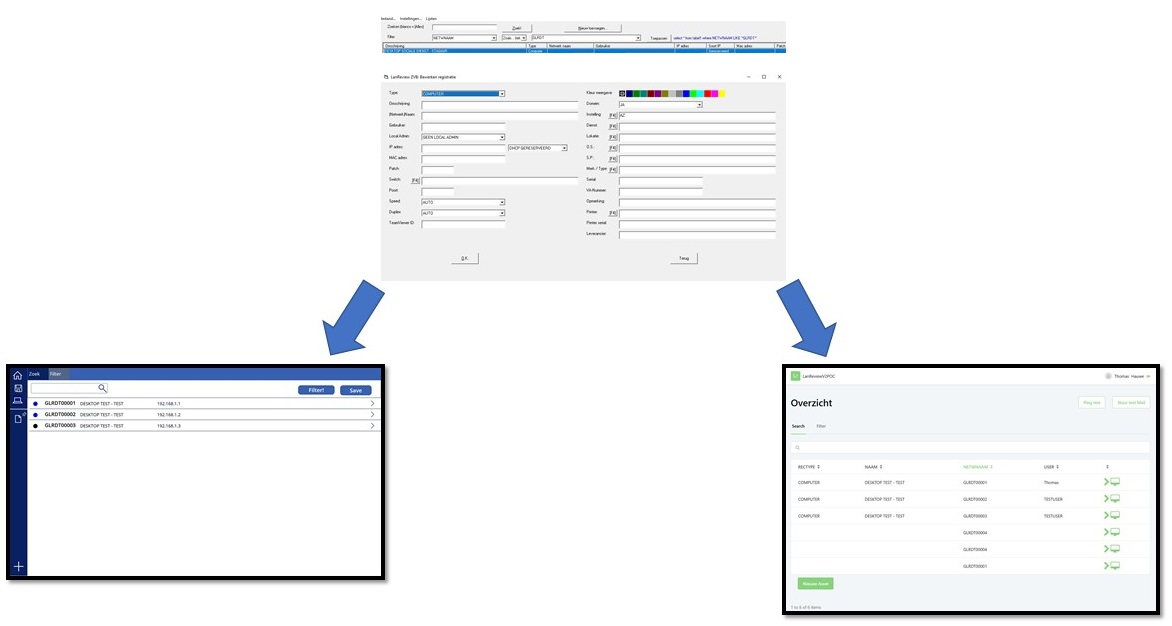
\includegraphics[width=1.0\linewidth]{poc-tri}
    \captionof{figure}{\color{HoGentAccent5} Voorbeeldweergaven van de proof-of-concepts.}
\end{center}\vspace{1cm}

%------------------------------------------------



\color{HoGentAccent1} 
\section*{Conclusies}
\color{black}
Sommige requirements zijn eenvoudig uit te werken maar anderen hebben workarounds nodig die na uitwerking nog steeds tekort schoten tenopzichte wat de originele LanReview mogelijk was. Indien men tijdens de uitwerking van een app workarounds en custom connectors moet beginnen gebruiken is het daarom aangeraden om een andere weg uit te gaan. Door de nodige tijdsinvestering kan evengoed iets opgesteld worden in een traditionele ontwikkelomgeving en het sterkste voordeel van low-code is daarmee tenietgedaan.\\
Dit wil niet zeggen dat PowerApps geen meerwaarde biedt voor deze case. Voor het maken van een strikt mobiele versie met een beperktere functionaliteitsset is het zeer geschikt. Bijvoorbeeld voor een telefoonboek app zou het ook perfect zijn.

Voor het maken van een complexere business app is Outsystems de beste keuze. De leercurve is niet dermate hoger dan die van PowerApps en indien de app beperkte resources en gebruikersbestand nodig heeft moet bovendien geen betalend plan aangegaan worden. Dit is het geval voor de LanReview POC maar er zijn nog steeds beperkingen mogelijk door de aard van de applicatie (cloud). Als lokale resources nodig zijn is dit net als bij PowerApps een hekelpunt. Het besluit hierbij is dat als AZ Glorieux een complexe app nodig heeft Outsystems een goede optie is maar als vervanger van LanReview is het niet toereikend.

De meest passende oplossing voor het vernieuwen van de desktopversie van LanReview is om de broncode over te zetten naar een WPF of UWP .NET Core desktop applicatie of soortgelijk. 

\vspace{1cm}

Low-code (PowerApps) heeft wel degelijk een toekomst in AZ Glorieux maar er moet rekening gehouden worden met requirements:
\begin{itemize}
    \item Eenvoudige requirements $\rightarrow$ Low-code voor citizen developers (no-code) - \textbf{PowerApps}.
    \item Complexe requirements $\rightarrow$ Low-code voor ontwikkelaars - \textbf{Outsystems}.
    \item Specifieke requirements, grote integratie met host systeem nodig $\rightarrow$ Traditionele desktop app.
\end{itemize}
%----------------------------------------------------------------------------------------
%	FORTHCOMING RESEARCH
%----------------------------------------------------------------------------------------
\color{HoGentAccent1} 
\section*{Toekomstig onderzoek}
\color{black}

\begin{itemize}
    \item Case met AI Builder
    \item REST operaties de focus van het onderzoek maken.
    \item Een asset management app die ook IoT devices opneemt.
\end{itemize}


%----------------------------------------------------------------------------------------

\end{multicols}
\end{document}